\documentclass{article}

% Packages
\usepackage{graphicx}
\usepackage{listings}
\usepackage{xcolor}
\usepackage{hyperref}

% Define code style
\lstdefinestyle{mystyle}{
    backgroundcolor=\color{white},
    commentstyle=\color{green},
    keywordstyle=\color{blue},
    numberstyle=\tiny\color{gray},
    basicstyle=\ttfamily\small,
    breakatwhitespace=false,
    breaklines=true,
    captionpos=b,
    keepspaces=true,
    numbers=left,
    numbersep=5pt,
    showspaces=false,
    showstringspaces=false,
    showtabs=false,
    tabsize=2
}

% Set code style
\lstset{style=mystyle}

\begin{document}

% Title
\title{Federated Learning Project Report}
\author{Katta Sathwik \\ 20mcme16}
\date{\today}
\maketitle

% Table of Contents
\tableofcontents
\newpage

% Abstract
\begin{abstract}
    This report presents a detailed analysis of a Log Anomaly Detection using federated learning project focusing on sequence classification using a fine-tuned BERT model. The project involves client-server communication using Flower framework for federated learning. This report outlines the key concepts and tasks involved in the implementation.
\end{abstract}

% Introduction
\section{Introduction}
Federated learning is a distributed machine learning approach that allows training models across decentralized devices or servers. In this project, I have used the Flower framework for federated learning to implement the solution for sequence classification. The model used is a fine-tuned BERT (Bidirectional Encoder Representations from Transformers) model, a state-of-the-art transformer-based architecture.

% Objective
\section{Objective}
The main objective of the project is to implement a federated learning system for sequence classification. The client-side code defines a Flower client using NumPyClient. The client utilizes a custom BERT model for sequence classification and a tokenizer for text encoding. The model is fine-tuned on a dataset and saved for later use.

% Section: Explanation of Model
\section{Explanation of Model}
The implementation of federated learning using the Flower framework is explained. Here are the key points:

\subsection{Starting the Flower Server}
\begin{enumerate}
    \item \texttt{fl.server.start\_server} is called to start the Flower server. It listens on a specific address and port (localhost and the port specified as a command-line argument).
    \item \texttt{ServerConfig} is used to configure the server with the number of federated learning rounds (\texttt{num\_rounds}) and the maximum message length.
\end{enumerate}

\subsection{Flower Client Implementation}
\begin{enumerate}
    \item Initially, import the necessary libraries for the implementation:
    \begin{itemize}
        \item \texttt{flwr} for federated learning.
        \item \texttt{tensorflow} and \texttt{keras} for machine learning and neural network models.
        \item \texttt{sys} to access command-line arguments.
        \item \texttt{numpy} for numerical operations.
    \end{itemize}
    \item Define auxiliary methods:
    \begin{itemize}
        \item \texttt{getDist}: Meant for visualizing data class distribution.
        \item \texttt{getData}: Customize the data distribution.
    \end{itemize}
    \item Load and compile the Keras model:
    \begin{itemize}
        \item Define a neural network model using the Keras Sequential API. It's a simple feedforward model with three layers: input, hidden, and output layers.
        \item Compile the model with an optimizer (\texttt{"adam"}), a loss \\ function (\texttt{"sparse\_categorical\_crossentropy"}), and a metric to track (\texttt{"accuracy"}).
    \end{itemize}
    \item Load the dataset:
    \begin{itemize}
        \item Load the Fashion MNIST dataset using TensorFlow's built-in dataset loader.
        \item Normalize the images to values between 0 and 1.
        \item Specify a data distribution (\texttt{dist}) for Fashion MNIST. This distribution controls how many samples are included from each class (0-9).
    \end{itemize}
    \item Define the Flower client:
    \begin{itemize}
        \item Define a custom Flower client class, \texttt{CustomClient}, which extends \texttt{fl.client.NumPyClient}.
        \item Implement three main methods:
        \begin{enumerate}
            \item \texttt{get\_parameters}: Returns the current model's weights.
            \item \texttt{fit}: Used for model training. Receives model parameters, updates the model, and fits the model to the training data for one epoch. Returns the updated model parameters and the number of training samples used.
            \item \texttt{evaluate}: Evaluates the model on the test data and returns the loss and accuracy.
        \end{enumerate}
    \end{itemize}
    \item Start the Flower client:
    \begin{itemize}
        \item \texttt{fl.client.start\_numpy\_client} is used to start the Flower client.
        \item It connects to the Flower server at the specified address.
        \item Use the custom client class (\texttt{CustomClient}), and set the maximum message length to ensure compatibility with the server.
    \end{itemize}
\end{enumerate}

\subsection{Fashion MNIST Dataset}
Fashion MNIST is a dataset commonly used in machine learning and computer vision tasks, often serving as a drop-in replacement for the original MNIST dataset. Instead of handwritten digits, Fashion MNIST contains grayscale images of various clothing items and accessories. Here's an explanation of the Fashion MNIST dataset:

\subsubsection{Images}
Fashion MNIST consists of a collection of \(28 \times 28\)-pixel grayscale images. Each image represents one of ten different fashion categories.

\subsubsection{Classes}
There are ten classes, each corresponding to a specific type of clothing item or accessory. These classes are as follows:

\begin{enumerate}
    \item T-shirt/top
    \item Trouser
    \item Pullover
    \item Dress
    \item Coat
    \item Sandal
    \item Shirt
    \item Sneaker
    \item Bag
    \item Ankle boot
\end{enumerate}

\subsubsection{Size}
The dataset is relatively small compared to some other image datasets. It includes 60,000 training images and 10,000 test images.

% Section: Basic Implementing a Federated Learning Setup
\section{Basic Implementing a Federated Learning Setup using Terminals as Clients with FashionMNIST Dataset}

% Subsection: Starting the Flower Server
\subsection{Starting the Flower Server}
To start the Flower server, use the following command in the terminal:

\begin{lstlisting}[language=sh, caption={Starting the Flower Server}]
fl.server.start_server --server_address="127.0.0.1:5012" --num_rounds=5 --max_msg_len=1000000
\end{lstlisting}

% Subsection: Starting Flower Clients
\subsection{Starting Flower Clients}
Open multiple terminals and run the Flower clients using the following command:

\begin{lstlisting}[language=sh, caption={Starting Flower Clients}]
python fashion_mnist_client.py --server_address="127.0.0.1:5012"
\end{lstlisting}

Ensure that Flower clients are running on different terminals to simulate a federated learning environment.

% Placeholder for Screenshots
\begin{figure}[h]
    \centering
    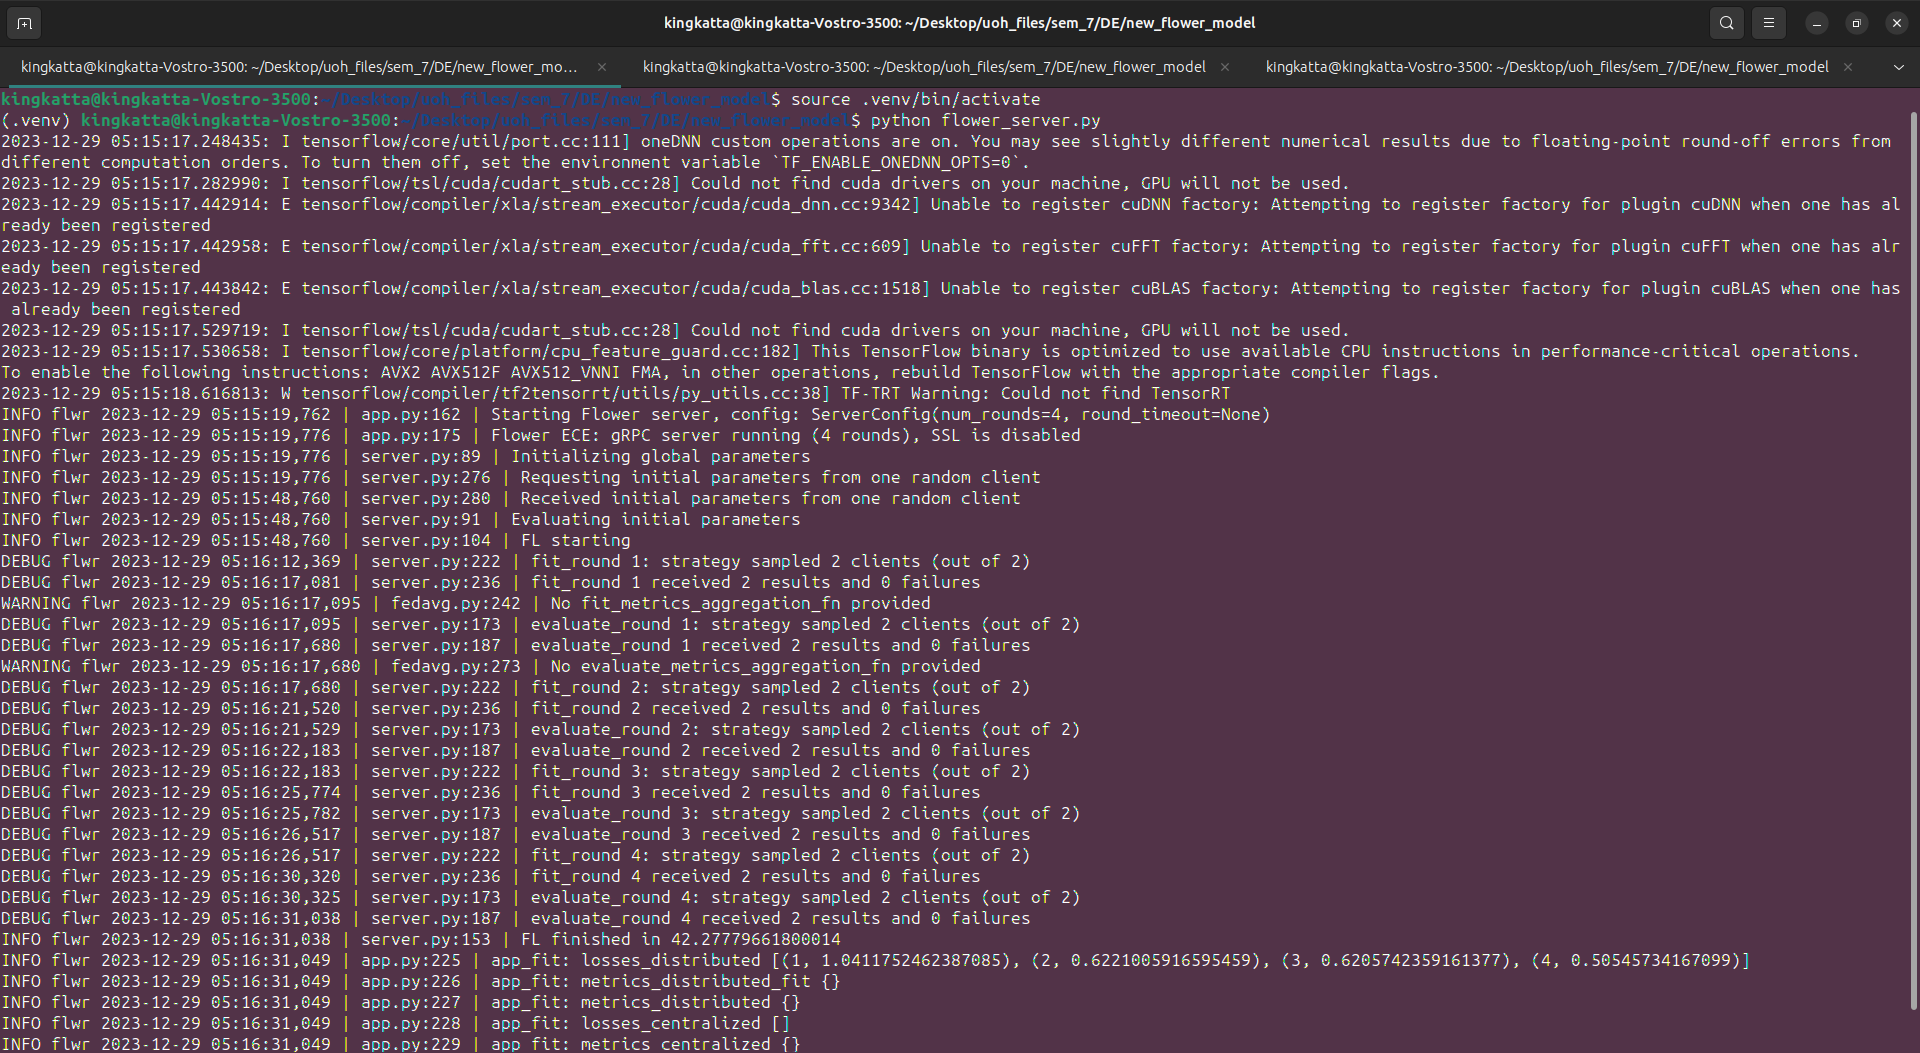
\includegraphics[width=0.9\textwidth]{server.png}
    \caption{Output of the server}
    \label{Output of the server}
    
    \vspace{\floatsep} % Add some vertical space between the figures
    
    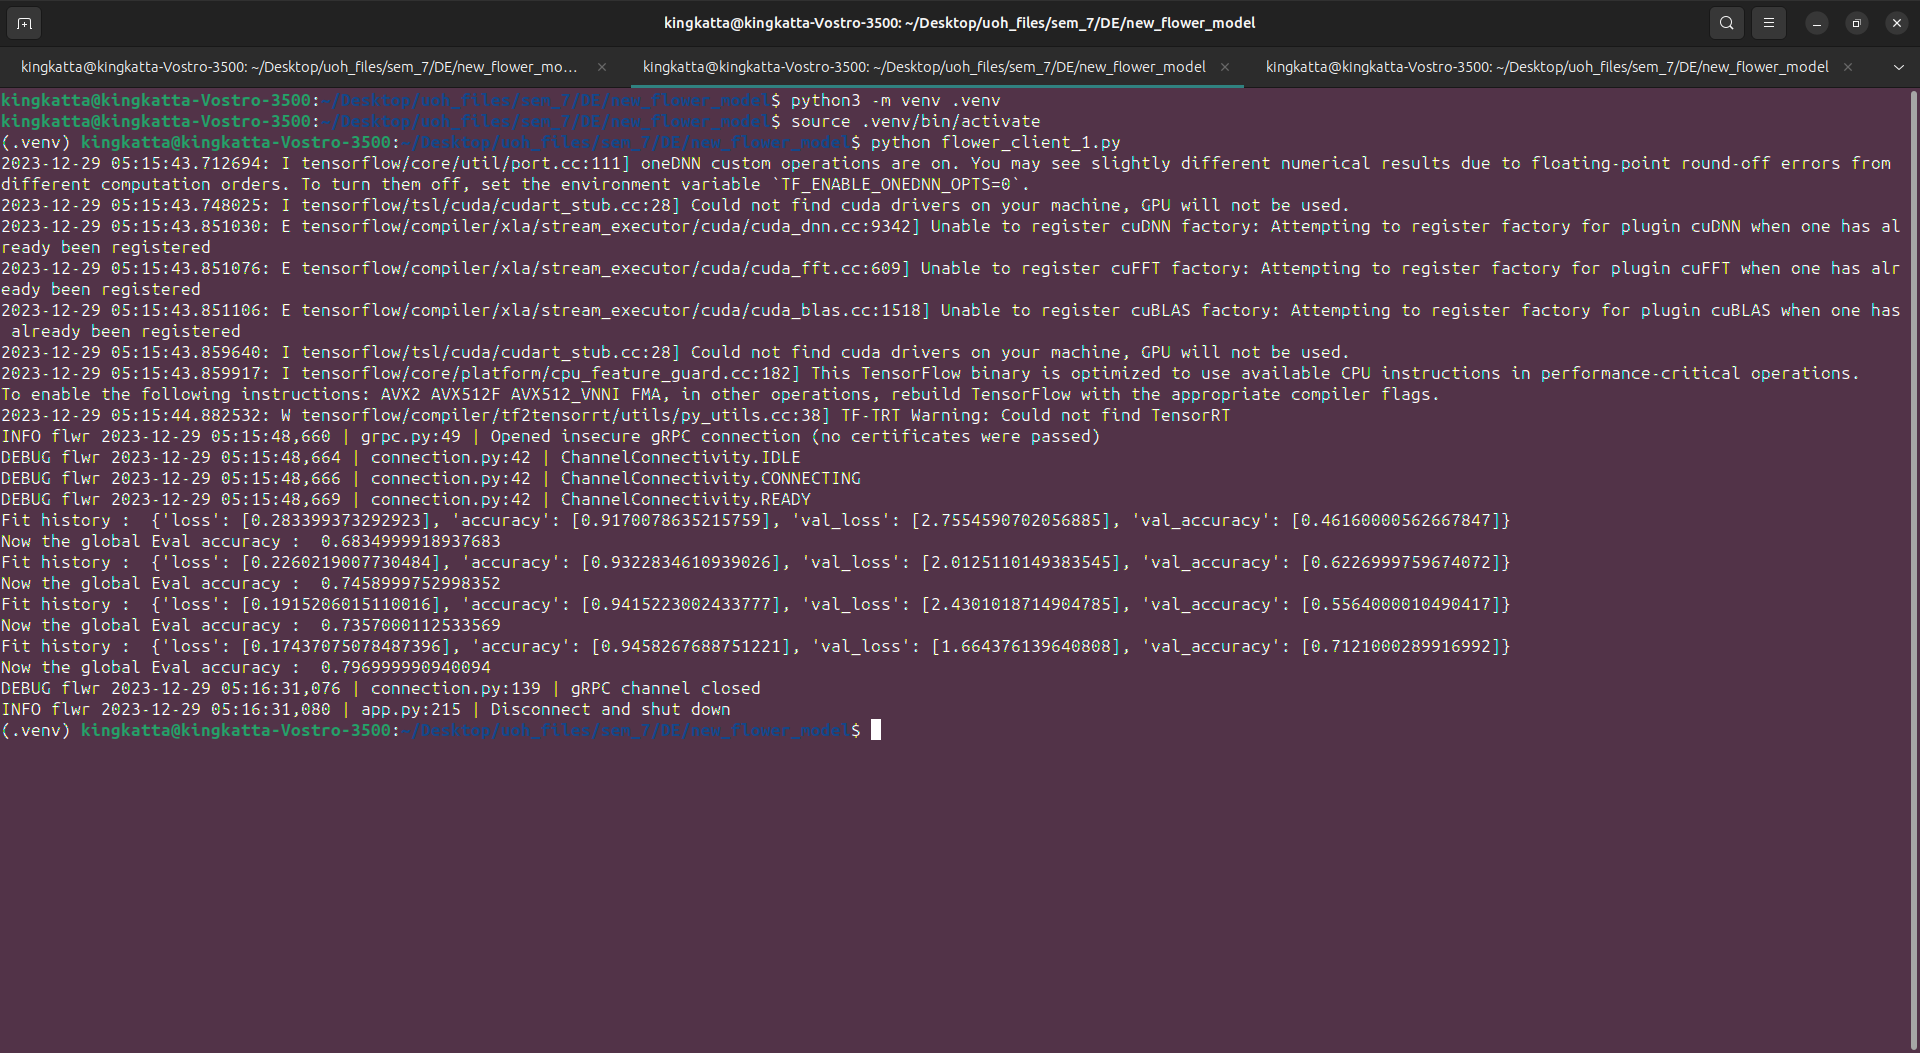
\includegraphics[width=0.9\textwidth]{client_1.png}
    \caption{Output of client 1}
    \label{Output of client 1}
    
    \vspace{\floatsep} % Add some vertical space between the figures
    
    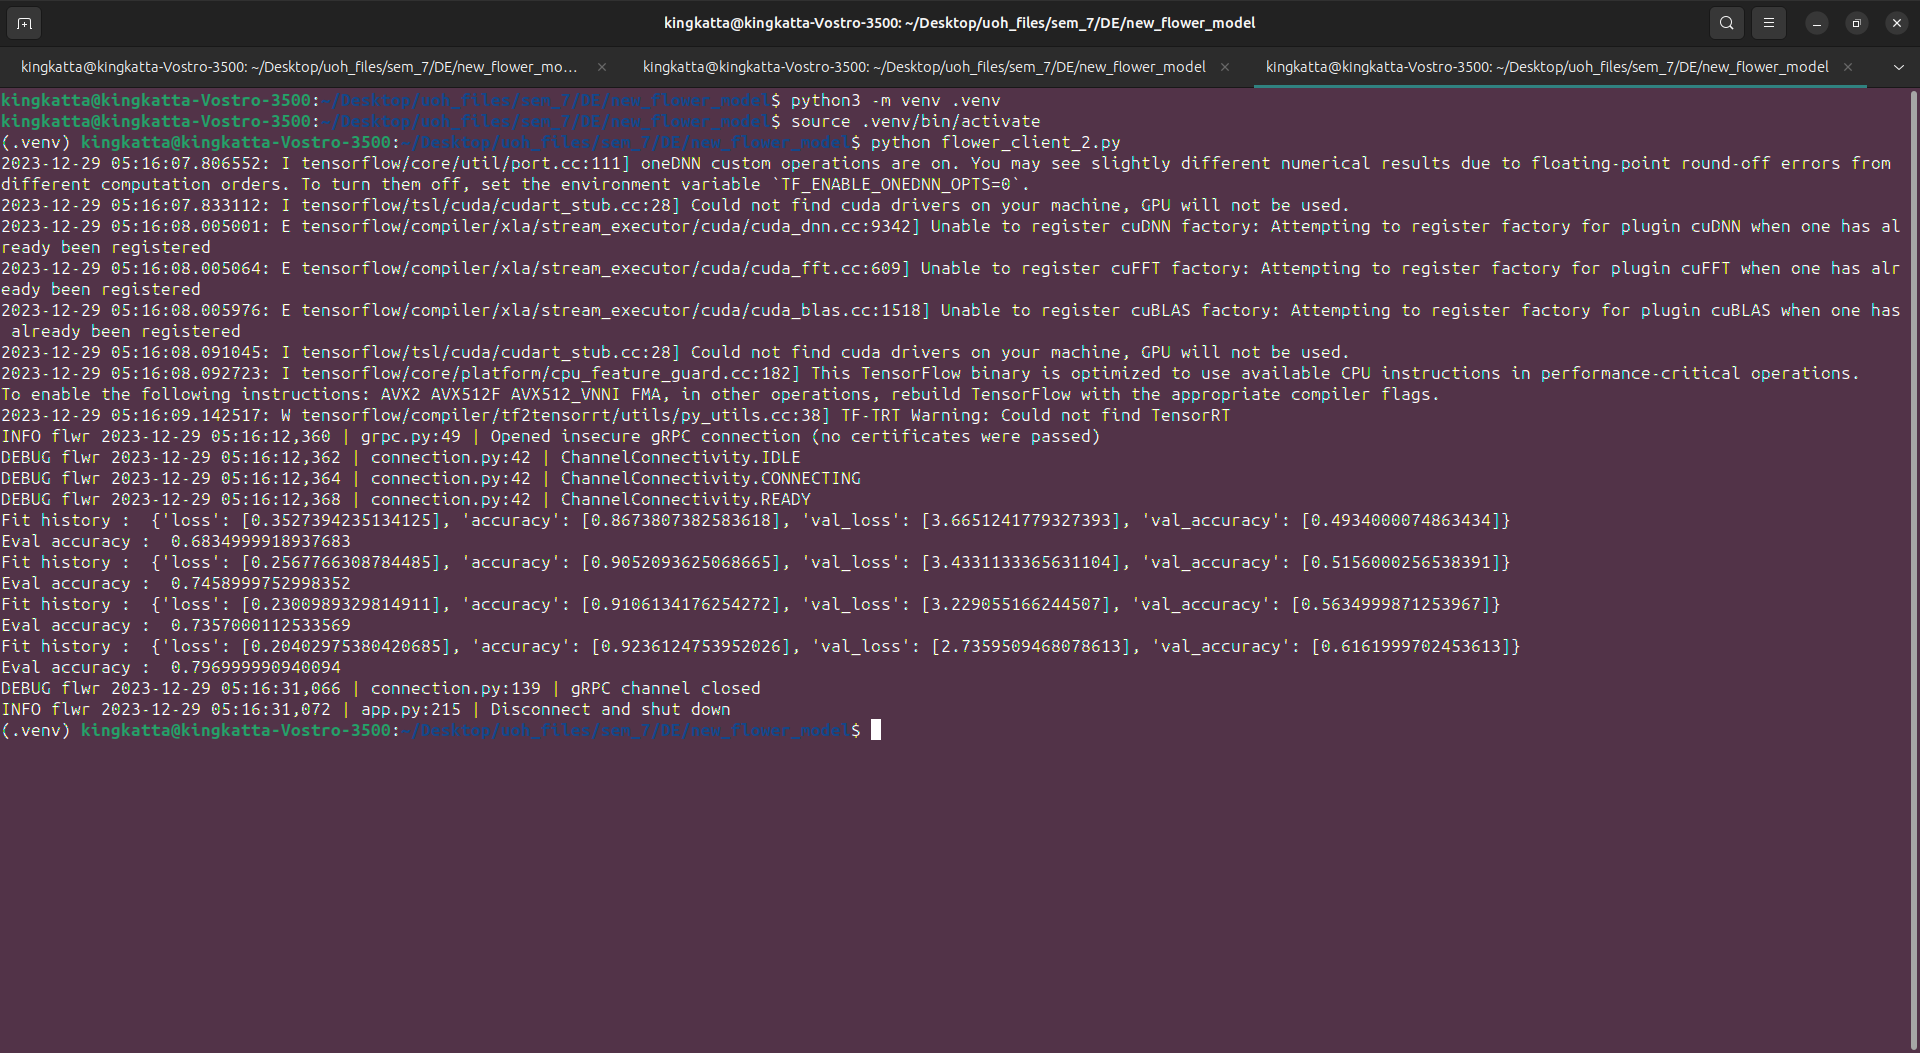
\includegraphics[width=0.9\textwidth]{client_2.png}
    \caption{Output of client 2}
    \label{Output of client 2}
\end{figure}

\section{Federated client for aggregation}
\subsection{Importing the necessary libraries}
These lines import necessary libraries and modules for working with PyTorch, Flower (Federated Learning framework), Hugging Face Transformers (for BERT), and other utilities.
% Placeholder for Code Snippets
\begin{lstlisting}[language=Python, caption={Hdfs Client for aggregation}, label=code:Hdfs client]
from dataclasses import dataclass
from typing import Any, Dict, List, Union
import torch
import flwr as fl
from transformers import BertForSequenceClassification, BertTokenizer, Trainer, TrainingArguments
from transformers import AdamW, get_linear_schedule_with_warmup
import torch.nn.functional as F
from torch.utils.data import Dataset, DataLoader
import zipfile
import pandas as pd
import shutil
import os
from sklearn.model_selection import train_test_split
\end{lstlisting}

\subsection{Custom Dataset Class:}
This class defines a custom dataset for PyTorch. It takes encodings (tokenized input sequences) and labels and provides methods for getting items and the length of the dataset.

\begin{lstlisting}[language=Python]
class CustomDataset(Dataset):
    def __init__(self, encodings, labels):
        self.encodings = encodings
        self.labels = labels

    def __getitem__(self, idx):
        item = {key: torch.tensor(val[idx]) for key, val in self.encodings.items()}
        item['labels'] = torch.tensor([self.labels[idx], 1 - self.labels[idx]]).float()
        return item

    def __len__(self):
        return len(self.labels)
\end{lstlisting}

\subsection{Initialization and Data Preprocessing:}
This section initializes the BERT model and tokenizer and loads a labeled dataset from a CSV file. It selects a subset of the dataset (rows 1 to 200) and preprocesses the data.

\begin{lstlisting}[language=Python]
model_saved = BertForSequenceClassification.from_pretrained("bert-base-uncased")
tokenizer_saved = BertTokenizer.from_pretrained("bert-base-uncased")
model_folder = "fine_tuned_bert_model_for_HDFS"
pickle_file = "pickle_fine_tuned_bert_model_for_HDFS.pickle"
df = pd.read_csv('Hdfs_labelled_sequence.csv', sep=',', quotechar='"', names=["text", "label"])
df = df[1:200]
X = list(df['text'])
y = pd.get_dummies(df['label'], drop_first=True)['Normal'].values
y = y.astype(int)
\end{lstlisting}

\subsection{Model Saving and Loading:}
This part saves the initial BERT model's weights and then loads the saved weights from a ZIP file. It ensures that the model and tokenizer are initialized with the same state as before saving.

\begin{lstlisting}[language=Python]
torch.save(model_saved.state_dict(), os.path.join(model_folder, "model_weights.pth"))
shutil.make_archive(model_folder, 'zip', model_folder)
with zipfile.ZipFile(f"{model_folder}.zip", "r") as zip_ref:
    with zip_ref.open("model_weights.pth", "r") as file:
        model_weights = torch.load(file)
model_saved = BertForSequenceClassification.from_pretrained("bert-base-uncased")
model_saved.load_state_dict(model_weights)
tokenizer_saved = BertTokenizer.from_pretrained("bert-base-uncased")
\end{lstlisting}

\subsection{Training Arguments and Trainer Initialization:}
Here, training arguments for the Trainer are defined, specifying various parameters like batch size, evaluation steps, etc. The Trainer is then initialized with the BERT model, training arguments, and training and evaluation datasets.

\begin{lstlisting}[language=Python]
training_args = TrainingArguments(
        output_dir="./bert_base_model",
        evaluation_strategy="steps",
        eval_steps=100,
        per_device_train_batch_size=2,
        per_device_eval_batch_size=2,
        save_steps=1000,
        save_total_limit=2,
        num_train_epochs=10,
        logging_dir="./logs",
    )
trainer = Trainer(
    model=model_saved,
    args=training_args,
    train_dataset=dataset_train,
    eval_dataset=test_dataset,
    data_collator=None
)
\end{lstlisting}


\subsection{FlowerClient Class:}
This class is a custom client for federated learning using the Flower framework. It has methods for getting parameters, fitting the model, and evaluating the model, among others.

\begin{lstlisting}[language=Python]
class FlowerClient(fl.client.NumPyClient):
    ...
\end{lstlisting}

\subsection{Fitting the Model (Training):}
loop runs the training process for a specified number of epochs. It iterates through batches of the local dataset, computes the loss, performs backpropagation, and updates the model parameters.

\begin{lstlisting}[language=Python]
for epoch in range(3):
    for batch in DataLoader(test_dataset, batch_size=2, shuffle=True):
        ...
\end{lstlisting}

\subsection{Evaluating the Model:}
This loop runs the evaluation process on the local dataset. It computes the loss and evaluates the model's performance.

\begin{lstlisting}[language=Python]
for batch in DataLoader(test_dataset, batch_size=2, shuffle=False):
    ...
\end{lstlisting}

\subsection{Printing Fit History and Evaluation Metrics:}
These print statements provide information on the fit history (training loss) and evaluation metrics (evaluation loss and global evaluation accuracy).

\begin{lstlisting}[language=Python]
print("Fit history: {'loss':", loss.item(), "}")
print("Evaluation metrics: {'eval_loss':", average_loss, "}")
print("Now the global Eval accuracy:", 1.0 - average_loss)
\end{lstlisting}

\subsection{Flower Client Initialization and Execution:}
The script starts the Flower client, connecting it to a server address and using the custom FlowerClient for federated learning.

\begin{lstlisting}[language=Python]
if __name__ == '__main__':
    fl.client.start_numpy_client(
        server_address="127.0.0.1:5020",
        client=FlowerClient(),
    )
\end{lstlisting}

% Section: HDFS Trained Model Aggregation With Federated Learning
\section{HDFS Trained Model Aggregation With Federated Learning}
Initially, I have worked on the HDfs trained model in order to aggregate the model using the federated learning, which automatically works for the aggregating three trained models but that was taking too long and more ram even if take a small amount of data for preprocessing.

% Placeholder for Screenshots
\begin{figure}[h]
    \centering
    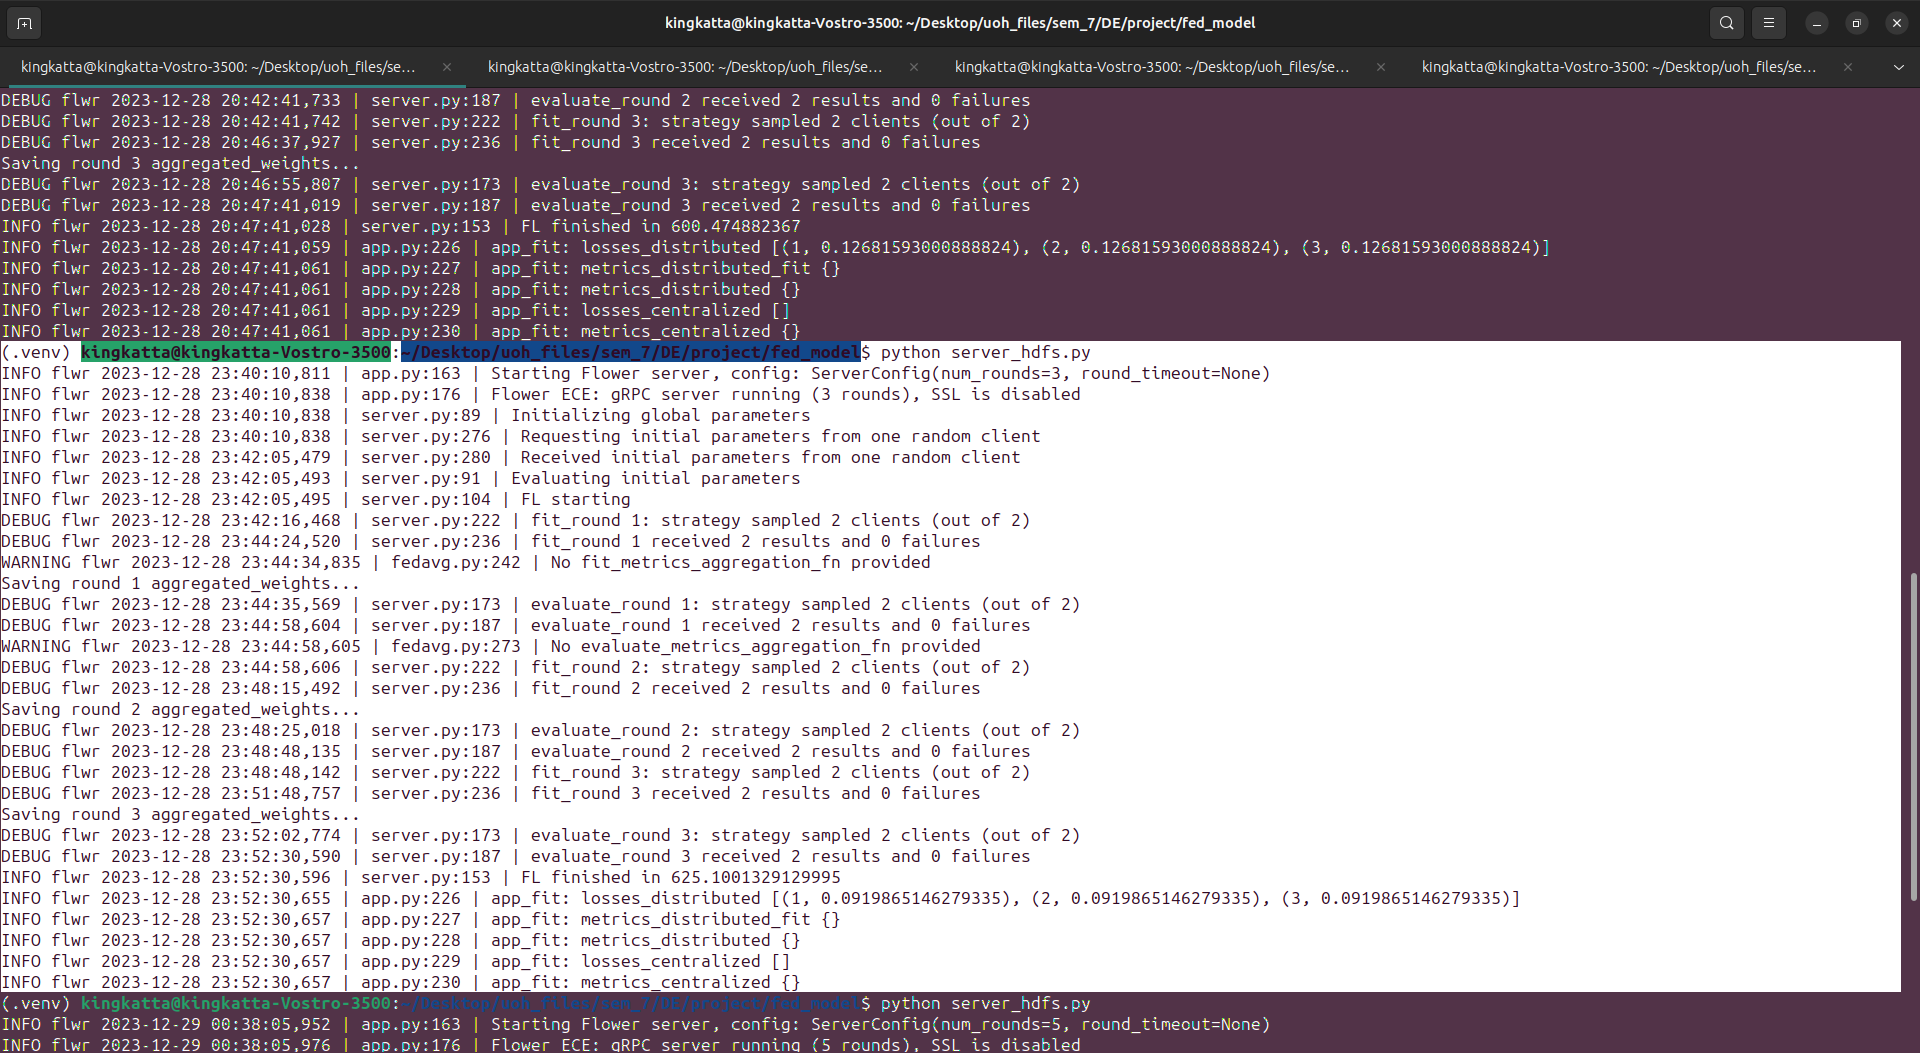
\includegraphics[width=0.9\textwidth]{hdfs_server.png}
    \caption{Hdfs Server}
    \label{Hdfs Server}
    
    \vspace{\floatsep} % Add some vertical space between the figures
    
    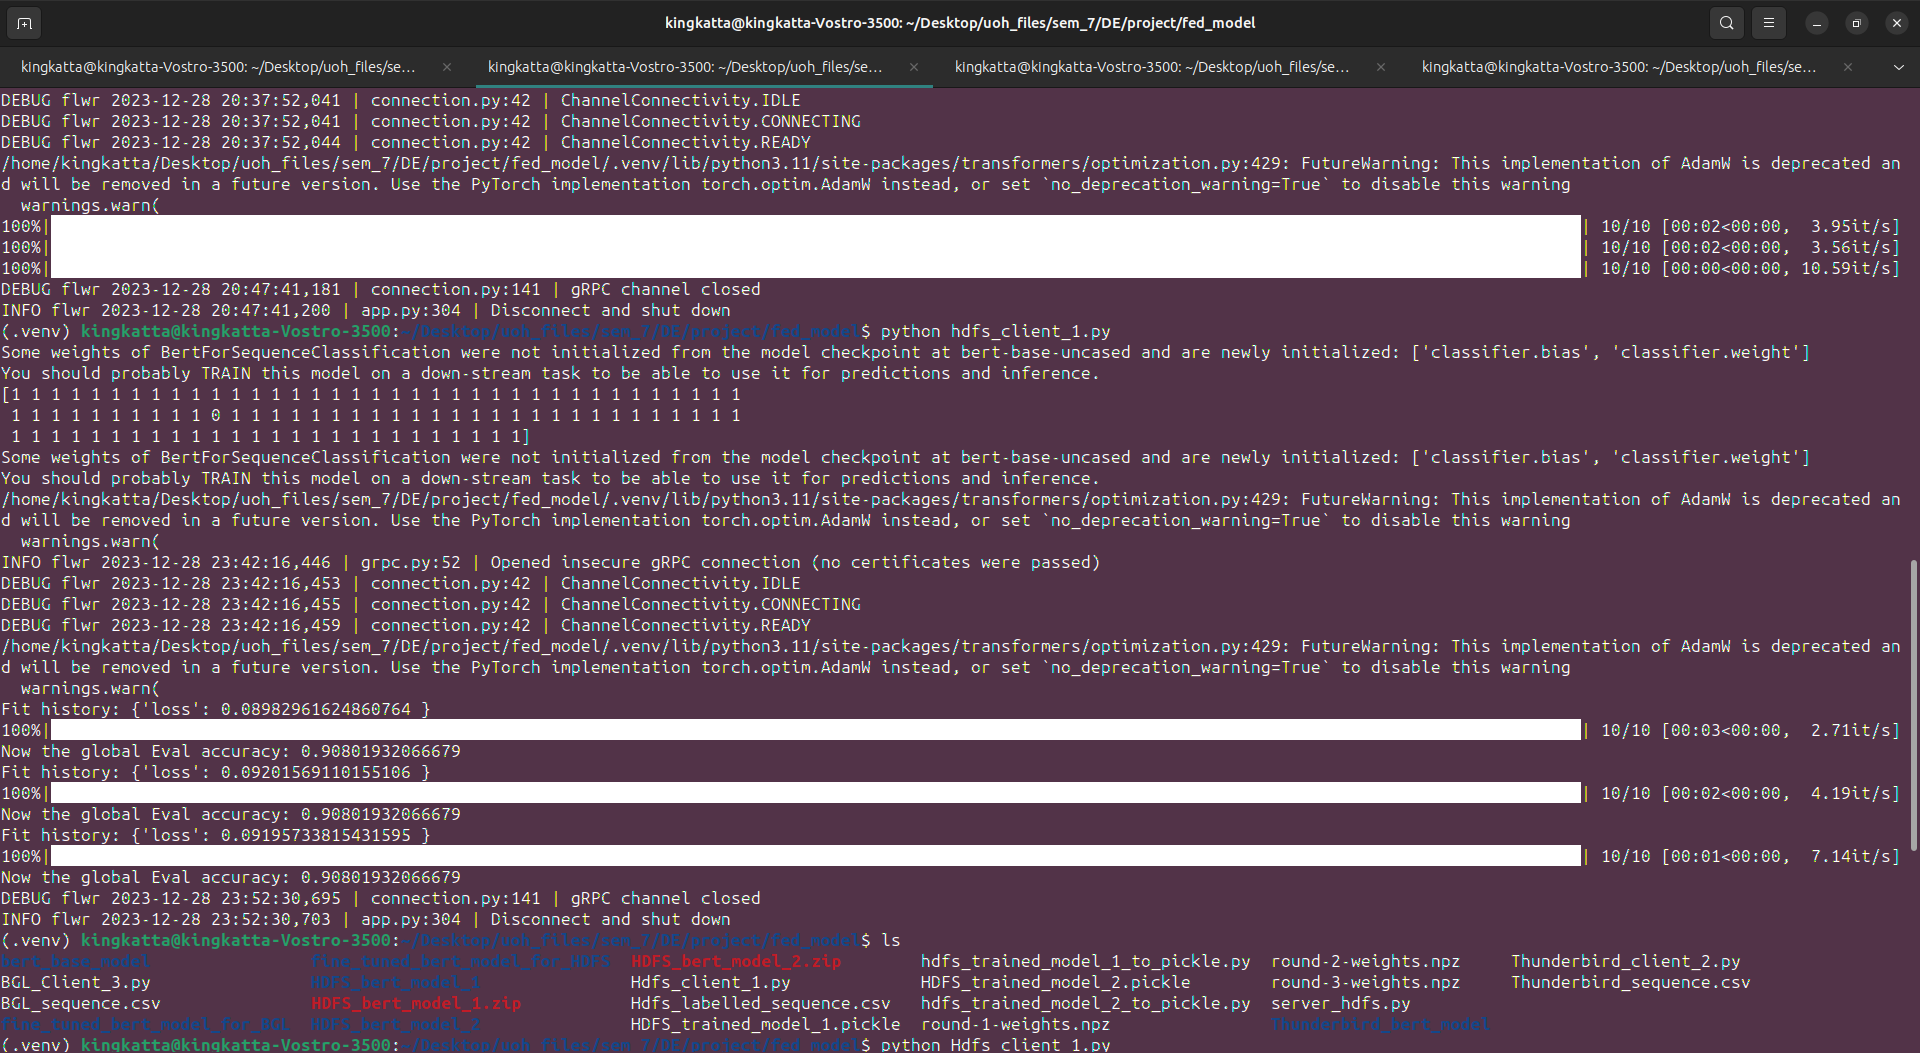
\includegraphics[width=0.9\textwidth]{hdfs_client_1.png}
    \caption{Hdfs Client 1}
    \label{Hdfs Client 1 Output}
    
    \vspace{\floatsep} % Add some vertical space between the figures
    
    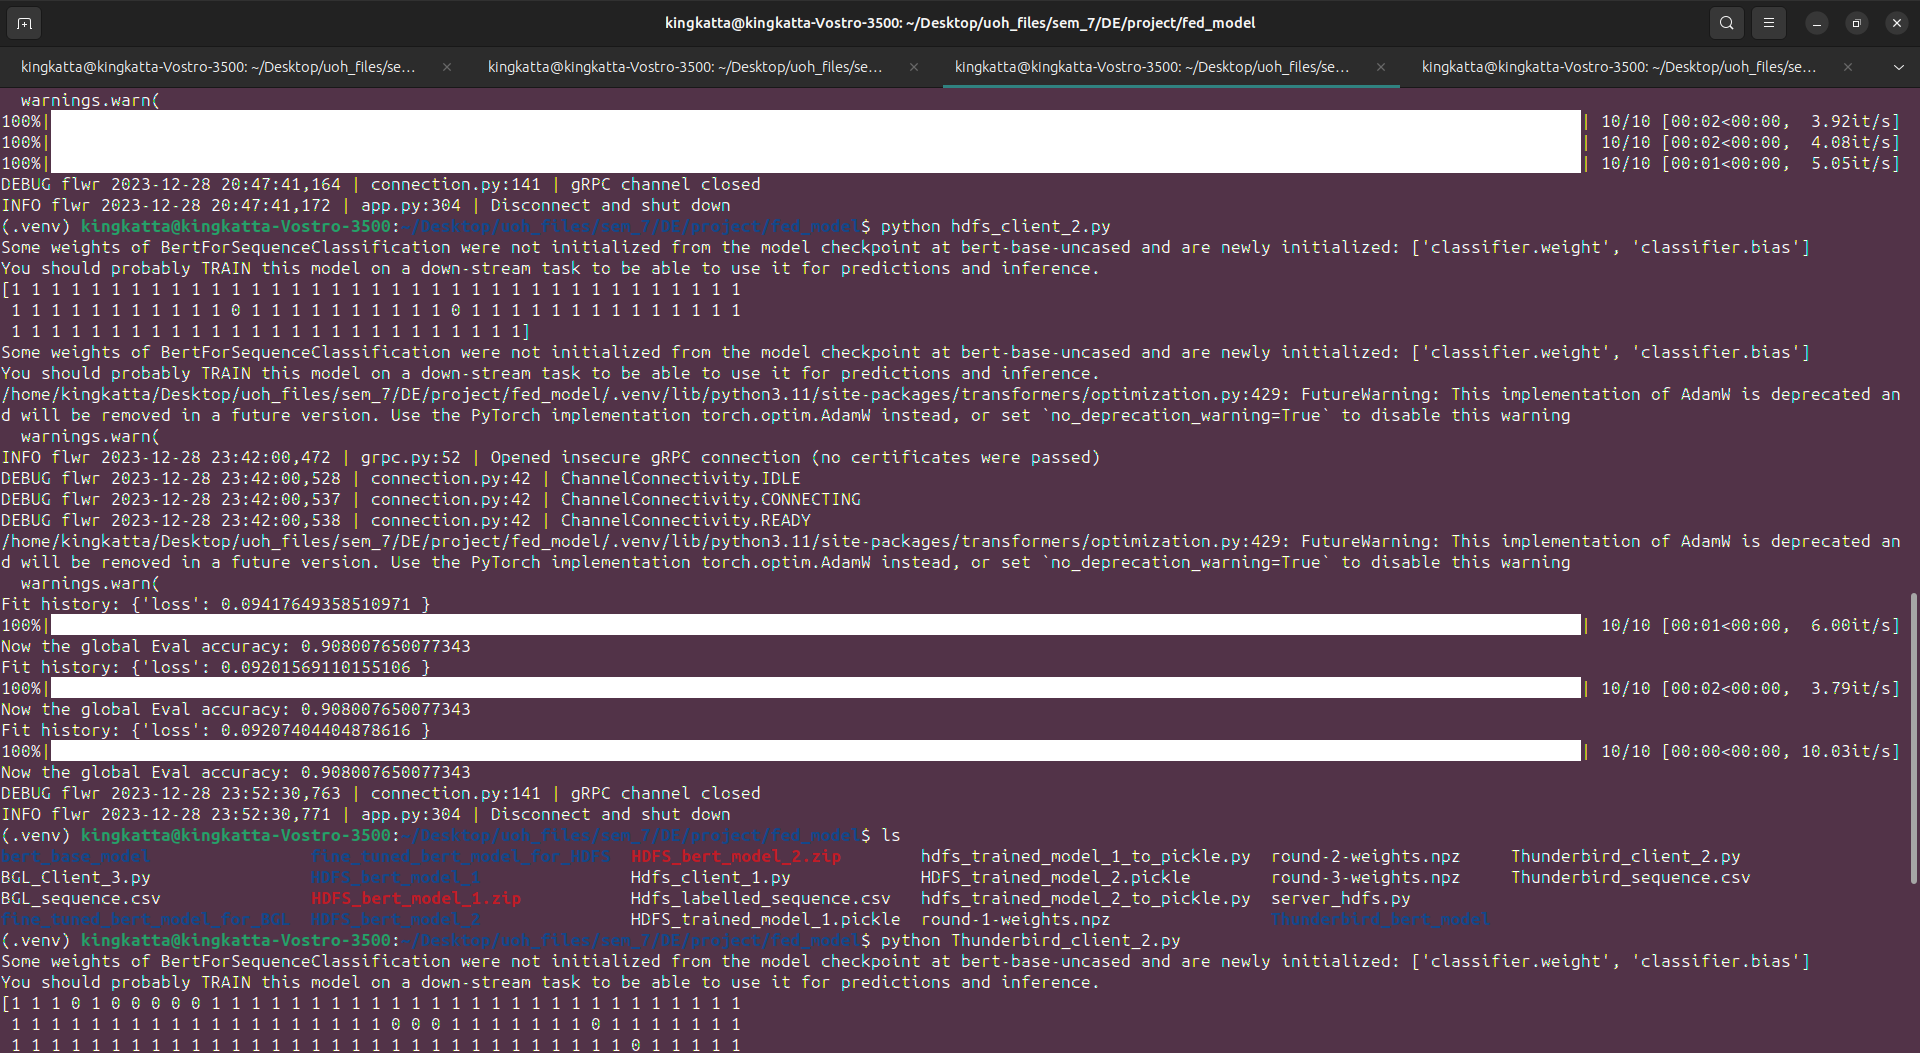
\includegraphics[width=0.9\textwidth]{hdfs_client_2.png}
    \caption{Hdfs Client 1}
    \label{Hdfs Client 1 Output}
    
\end{figure}

% Placeholder for Screenshots
\begin{figure}[h]
    \centering
    
    \vspace{\floatsep} % Add some vertical space between the figures
    
    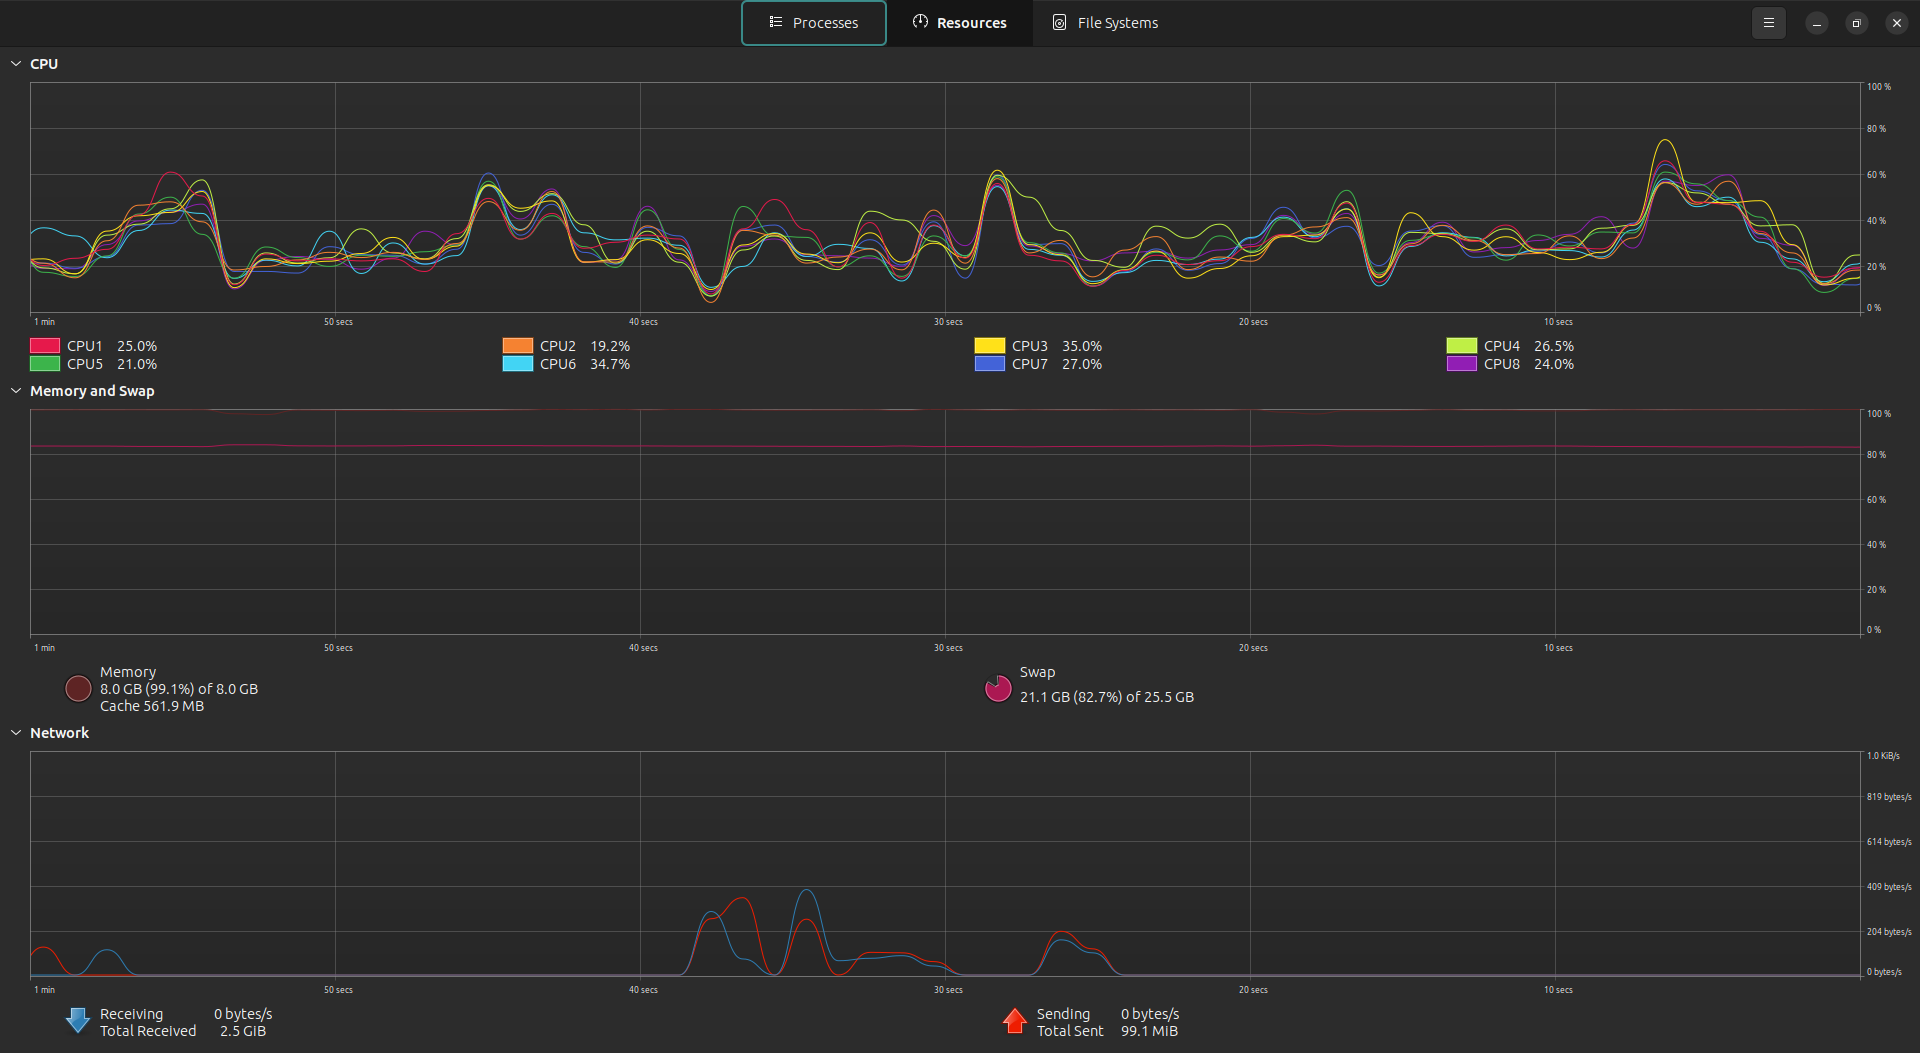
\includegraphics[width=0.9\textwidth]{ram.png}
    \caption{Ram usage while Training}
    \label{Ram usage while Training}
\end{figure}

% Conclusion
\section{Conclusion}
This report demonstrates federated learning with BERT using the Flower framework. It includes data preprocessing, model saving/loading, training, and evaluation in a federated learning setup. The Flower client facilitates communication between the server and clients for federated learning. The provided print statements offer insights into the training and evaluation processes.

\section{Reference}
\href{https://github.com/sushanthk-262/Log anomaly detection}{https://github.com/sushanthk-262/Log anomaly detection}

\end{document}
